\documentclass[tikz]{standalone}
\usepackage{tikz}
\usetikzlibrary{positioning,trees,decorations.pathreplacing}

\begin{document}
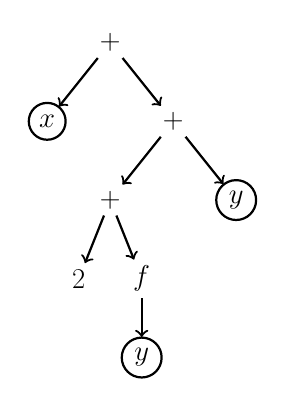
\begin{tikzpicture}[->,thick,scale=0.5, every node/.style={scale=0.5}
  , grow via three points={
      one child at (0,-2) and 
      two children at (.8,-2) and (-0.8,-2) 
  }]
     \tikzstyle{tnode}=[rectangle, inner sep=1.5mm]
     \tikzstyle{var}=[ circle, inner sep=1.5mm,draw]
     \def\rstep{5cm}
     \huge
         
    \begin{scope}[xshift= \rstep]
      \node[tnode] {$+$}
          child {node[tnode] {$+$} 
            child {  node[var] {$y$} }
            child[missing] {}
            child { node [tnode] {$+$}
                    child { node [tnode] {{$f$}} 
                                   child { node[var] {{$y$}} } }
                    child { node[tnode] {{2}} }
                   }
          }
          child[missing] {}
            child{ node [var] {{$x$}} 
            };
      \end{scope}
\end{tikzpicture}



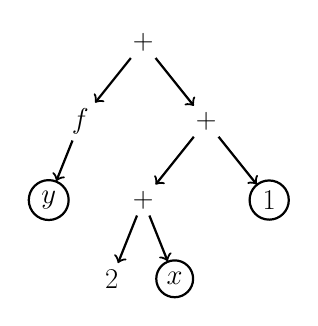
\begin{tikzpicture}[->,thick,scale=0.5, every node/.style={scale=0.5}
  , grow via three points={
      one child at (0,-2) and 
      two children at (.8,-2) and (-0.8,-2) 
  }]
     \tikzstyle{tnode}=[rectangle, inner sep=1.5mm]
     \tikzstyle{var}=[ circle, inner sep=1.5mm,draw]
     \def\rstep{5cm}
     \huge
         
    \begin{scope}[xshift=\rstep]
      \node[tnode] {$+$}
          child {node[tnode] {$+$} 
            child { node[var] {{1}} }
            child[missing] {}
            child { node [tnode] {$+$}
                    child{  node[var] {$x$} 
                    }
                    child { node[tnode] {{2}} }
                   }
          }
          child[missing] {}
            child{ node [tnode] {$f$} 
              child[missing] {}
               child { node[var] {$y$} }
            };
      \end{scope}
\end{tikzpicture}
\end{document}

